\newcommand{\vecc}[1]{\vec{\mathbf{#1}}}

\subsection{Overview and Domain Reduction}
% Overview
%   - we make a compiler
% for a restricted problem domain
% we generate a large amount of code
% we replace the lambda function with a call to this code
% pure functions with numerical input
% ignore the effects of numerical machine precision
Our solution, \phlat, is a domain specific compiler that generates code for a conventional compiler (e.g. g++) to optimise and turn into machine instructions.
Our goals for \phlat are that it:
\begin{itemize}
    \item Supports a large range of problems
    \item Generates code that is faster than the current default code
    \item Provides a user friendly interface for entering problems
    \item Is practical to use (e.g. compile times are not too long)
\end{itemize}

\phlat will operate in a restricted domain, specifically a domain that supports the definition of \proc{Patch Update}, \proc{Numerical Ingredient} and \proc{Problem Definitions}.
We define \phlat{}'s domain as follows:
\begin{enumerate}
    \item All functions are pure functions
    \item All functions have a fixed number of inputs and outputs
    \item All functions contain a fixed number of operations \label{cond:fixed}
    \item Functions can be nested \label{cond:nested}
    \item Machine precision effects can be ignored
    \item No function contains control flow \label{cond:no-cf}
\end{enumerate}
Many of these conditions come naturally from (\ref{eq:fv-simple}), mathematical functions are pure, have a fixed number of inputs, and ignore machine precision effects.
Condition \ref{cond:fixed} comes from the observation that within \proc{Patch Update} there are no unbounded \lstinline{for} or \lstinline{while} loops, every loop can be unrolled at compile time.
Condition \ref{cond:nested} comes from nested structure of \proc{Patch Update}, the \proc{Numerical Ingredient} and \proc{Problem Definitions}.
Condition \ref{cond:no-cf} may at first seem the most restrictive condition.
User code in ExaHyPE currently contains control flow in the form of a \lstinline{switch} statement depending on the normal vector.
And the current implementation of \proc{Patch Update}, contains both \lstinline{for} and \lstinline{if} statements.
However, as we will discuss in Section \ref{sec:DAG} a majority, if not all, control flow can be hoisted to DAG (Directed Acyclic Graph) creation, hence this condition isn't as restrict as it first seems.
An exception to this are piecewise functions e.g.
\[
    f(x) = \begin{cases} g(x)  & \text{if } x<0.5 \\  h(x)  & \text{if } x\geq 0.5 \\\end{cases}
\]
these are not supported by \phlat.
As will be elaborated in Section \ref{sec:DAG}, DAGs are a fundamental feature in \phlat, as such we can give an alternative definition of \phlat{}'s domain as: any problem that can be described as a DAG.

At a very high level, \phlat takes an input DAG and compiles it to C++.
To do this, \phlat makes various transforms to the DAG and to an Intermediate Representation (IR) described in Section \ref{sec:IR}.
Additionally users can provide extra DAG and IR transformations if they wish.
An overview of \phlat{}'s architecture can be found in Figure \ref{fig:arch}.

\begin{figure}[h!]
    \begin{center}
        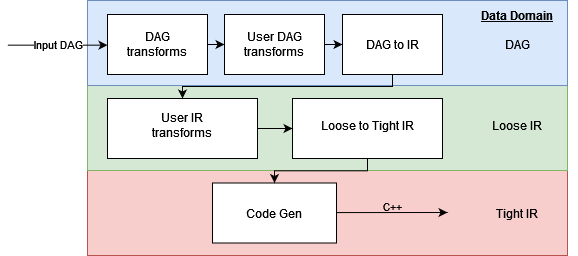
\includegraphics[width=.7
        \textwidth]{comp-arch.png}
        \caption{Overview of \phlat{}'s architecture.}
        \label{fig:arch}
    \end{center}
\end{figure}



\subsection{DAG} \label{sec:DAG}
% What is a DAG - chip model
% [ ] Explain chip model
% [ ] Show example
% [ ] Control flow hoisting

\phlat begins with a Directed Acyclic Graph (DAG) as an input.
The DAG model we propose takes inspiration from hardware design.
In a hardware design you define electrical components.
Each component has an ordered set of input and output ports and its output is a function of its input.
It is common, to also see test cases alongside a component to be used in verification.

In our DAG every node has a set of input and output ports.
Every input port must receive a single value and every output port can transmit copies of a single value.
Every node $n$ in our DAG describes a function: $\vecc{out ports}=n(\vecc{in ports})$ with the number of inputs and outputs being of a fixed length.

A node may be primitive and directly map to a primitive code operation, for example an addition node maps to $out_0 = in_0 + in_1$ (see Figure \ref{fig:bin_add}).
Or a node may be composite, where it is a DAG itself.
Composite nodes would map to functions in the final code output.
Figure \ref{fig:bn} demonstrates composite nodes with the calculation $out_0 = (in_0)^3 + in_1$ where the function \textit{cubed} has been implemented as a subgraph.
The nested structure provided by composite nodes gives our DAG model its expressive power and modularity.
For example, a user can create \proc{Problem Definition} DAGs, then pass those DAGs to pre-made \proc{Patch Update} and \proc{Numerical Ingredient} DAG builders to create a DAG that describes the full \proc{Patch Update} process.


\begin{figure}[h!]
    \begin{center}
        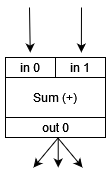
\includegraphics[width=.15\textwidth]{binary_add.png}
        \caption{Example of binary addition as a DAG node.}
        \label{fig:bin_add}
    \end{center}
\end{figure}

\begin{figure}[h!]
    \centering
    \subcaptionbox{Top level\label{fig:bn1}}{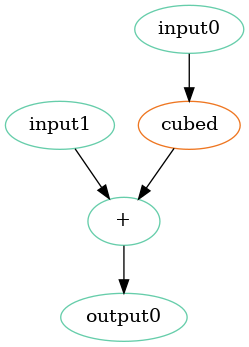
\includegraphics[width=.2\textwidth]{basic-nested-part1.png}}
    \hspace{1em}
    \subcaptionbox{Exploded view\label{fig:bn0}}{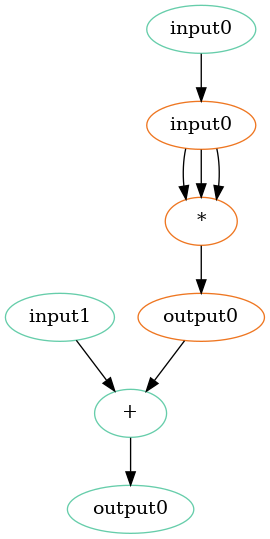
\includegraphics[width=.2\textwidth]{basic-nested-part0.png}}
    \caption{Example of a nested DAG that calculates $out_0 = (in_0)^3 + in_1$. The colour of a node is used to show if that node is composite or part of a composite node. NOTE. the visualisation displays a node's input edges in a random order.}\label{fig:bn}
\end{figure}

DAGs are created in Python.
Every type of node is a class.
To create a node you create an instance of the required class of node.
DAGs are a special type of node that implement additional functions.
Namely, DAG nodes store a sparse definition of the graph they represent and provide an interface for users to add edges to the graph.

Provided that our DAGs are indeed acyclic, we can always find an order to evaluate every internal node and thus process some given input.
In \phlat every node implements an \texttt{eval} function which takes an array of input values, applies that node's function to the input, and output the results.
This allows DAGs to be evaluated directly within Python opening up the door to writing unit and integration tests to verify DAGs.

The \texttt{eval} functions of all the primitive nodes are simple, often only preforming one operation.
The \texttt{eval} function for a DAG node is more complex, first calculating a valid traversal order of the DAG.
Following this traversal order, the DAG node calls the \texttt{eval} function on each internal node, forwarding the output evaluated nodes to the input of nodes yet to be processed.
This process repeats until the entire DAG has been traversed.

Using Python to create DAGs allows for the hoisting of control flow.
For example, take the a flux function used in an ExaHyPE project:
\begin{lstlisting}[language=c]
void flux(
  const double * __restrict__ Q, // input
  ...
  int normal,
  double * __restrict__ F // output
)  {
  switch(normal){  
  case 0: //in x direction
	  calc_flux_x(Q, ..., F)
	  break;
  case 1: //in y direction
	  calc_flux_y(Q, ..., F)
	  break;
  }  
}
\end{lstlisting}
The switch statement is run every evaluation of flux and depends on the value of the normal.
However, in \proc{Patch Update} the value of the normal is known at compile time.
Therefore, we can use a builder patten in python to hoist this control flow out of the flux function.
\begin{lstlisting}[language=python]
def build_flux_DAG(normal:int)->DAG:
    if normal==0:
        return build_flux_x_DAG()
    else:
        return build_flux_y_DAG()
\end{lstlisting}




\subsection{IR} \label{sec:IR}
% What is the IR - llvm inspired
% [ ] Explain IR
% [ ] Show example


DAGs are a natural way to express an input problem, however code generation directly from a DAG is challenging.
To overcome this issue we introduce an intermediate representation (IR).
The goal of this IR is to offer a middle ground between the DAG and output code.
It should be easy to transform the DAG into the IR, and it should be easy to transform this IR into code.
The IR we present takes inspiration from LLVM.
It is a set of function definitions, and within each function definition there is a linear sequence of instructions.

Variable management is the main code generation challenge we encounter.
\phlat supports interchangeable code generation backends, allowing different languages to be targeted.
This means it's preferable to include information such as variable declaration and complex function signatures in the IR, allowing code generation backends to stay as slim as possible.
However, the complications introduced by variable declarations and function signatures are a key reason why code generation directly from a DAG is hard.   


To combat these opposing requirements we create 2 standards for our IR.
The IR can be \textit{loose}, and the IR can be \textit{tight}.
When we transform our DAG we transform it into a loose IR.
A loose IR doesn't worry about variable declaration, variable declaration is implicit like in python.
There are also useful tools available in loose IRs such as a special class of temporary variables.
Additionally, loose function signatures are kept very simple.
A loose function maintains a list of (possibility hundreds) of single value input variables and a list of (possibly hundreds) of single value output variables.
The relaxed nature of the loose IR makes it ideal for preforming transforms and optimisations as there are few ways to invalidate a loose IR.

On the other hand, a tight IR is much stricter.
In a tight IR all variables must be named and declared.
And a tight function signature mirrors that of the target output code, containing a mixture of input and output variables that can be single values or arrays.
Figure \ref{fig:tight_loose} provides an example of loose and tight IR. 

\newsavebox{\looseIRlisting}
\begin{lrbox}{\looseIRlisting}% Store first listing
\minipage{.68\textwidth}
\begin{lstlisting}
define VOID @kernel (%in0, %in1) (%out0, %out1):
	%tmp1 = %in0
	%tmp2 = %tmp1 * %tmp1 * %tmp1
	%tmp3 = %in1
	%tmp4 = %tmp2 + %tmp3
	%tmp5 = %tmp4
	%tmp6 = %tmp2 - %tmp3
	%tmp7 = %tmp6
	%out0 = %tmp5
	%out1 = %tmp7
\end{lstlisting}
\endminipage
\end{lrbox}

\newsavebox{\tightIRlisting}
\begin{lrbox}{\tightIRlisting}% Store first listing
\minipage{.68\textwidth}
\begin{lstlisting}
define VOID @kernel (new #list(in), new #list(out)):
	new #tmp2 = #in[0] * #in[0] * #in[0]
	#out[0] = #tmp2 + #in[1]
	#out[1] = #tmp2 - #in[1]
	<return nothing>
\end{lstlisting}
\endminipage
\end{lrbox}

\begin{figure}
\centering

\sbox{\measurebox}{%
  \begin{minipage}{.68\textwidth} \centering
        \subfloat[Loose IR]{\label{fig:figB}\usebox{\looseIRlisting}}
        \vspace{1em}
        \subfloat[Tight IR]{\label{fig:figC}\usebox{\tightIRlisting}}
  \end{minipage}
}

\usebox{\measurebox}\qquad
    \begin{minipage}[][\ht\measurebox][c]{.26\textwidth}
      \subfloat[Input DAG]{\label{fig:loose_tight_dag}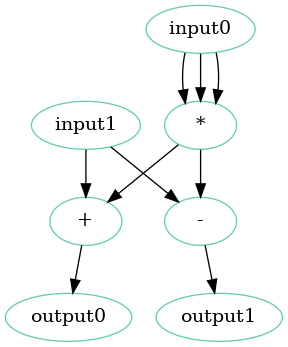
\includegraphics[width=\textwidth]{tight_vs_loose.png}}
       
    \end{minipage}
\caption{Example of the difference between a loose IR and tight IR. Figure \ref{fig:loose_tight_dag} shows the corresponding input DAG.}
\label{fig:tight_loose}
\end{figure}


\subsection{Compiler Architecture}
\phlat consists of 3 stages: the DAG transform stage; the IR transform stage; and the code generation stage.
An overview of \phlat{}'s architecture can be found in Figure \ref{fig:arch}
In the DAG transform stage a series of default transforms are applied to the DAG, followed optional user transforms.

\begin{figure}[h!]
    \centering
    \subcaptionbox{Nested DAG}{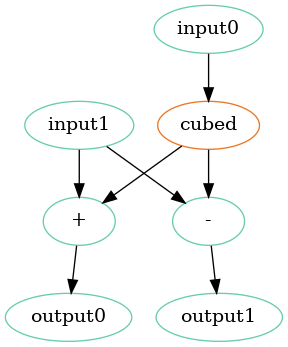
\includegraphics[width=.2\textwidth]{flatten-part1.png}}
    \hspace{1em}
    \subcaptionbox{Exploded view of nested DAG}{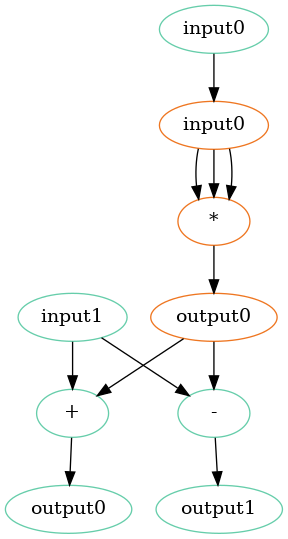
\includegraphics[width=.2\textwidth]{flatten-part0.png}}
    \hspace{1em}
    \subcaptionbox{Flattened DAG}{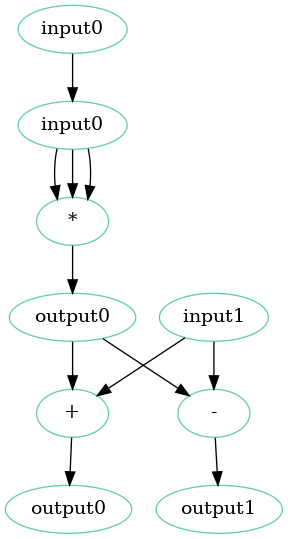
\includegraphics[width=.2\textwidth]{flatten-part2.png}}
    \caption{Example of the DAG flatten operation. Colours are used to indicated depth of nodes. Blue = depth 0, Orange = depth 1.}\label{fig:flatten_example}
\end{figure}

The most notable default transform is the flatten transform.
This transform takes a nested DAG (i.e. a DAG containing composite nodes) and for every composite node: the composite node is deleted and replaced by a copy of the DAG contained within the composite node.
Applied recursively, a highly nested DAG can be reduced to only contain primitive nodes, i.e. it is flattened.
This transform causes the final output code to be a single monolithic function, as opposed to a function containing many function calls.
An example of the flatten transform can be found in Figure \ref{fig:flatten_example}

A user transform we investigated was the removal of duplicated computation.
Within a DAG, duplicate computation manifests itself as 2 equivalent nodes (e.g. 2 addition nodes) that share the same inputs.
Once 2 such nodes are identified one can be deleted, and its output edges copied over to the node that remains.
Some care has to be taken if an operation is commutative (e.g. addition and max) or not (e.g. subtraction and division).

% DAG -> IR
Once all the DAG transforms are completed the DAG is transformed into the IR.
To do so, the DAG and every sub-DAG are identified and processed separately creating a set of loose functions.
Processing a DAG begins by creating a valid traversal order, much like DAG \texttt{eval} does.
Then following this order, every node in the DAG is transformed into an IR symbol.
Primitive nodes map to equivalent primitive IR Symbols and composite nodes map to loose IR function calls.
The output of every port of every node is stored as a new temporary variable, and these temporary variables are passed as the input to other nodes.
At the end of the transform we have an IR in loose form.

% IR Transforms 
The second stage of \phlat is the IR transform stage.
Interestingly there are equivalences between DAG transforms and IR transforms.
For example, the DAG transform \texttt{Remove Passthrough Nodes}, which removes all the primitive nodes that simply pass through a single value, is approximately equivalent to the IR transform \texttt{Remove Forward Aliasing}, which removes all lines that look like \lstinline{%tmp_x=%tmp_y} (i.e. a line that copies a single value).
However, it is not the case that all IR and DAG transforms share this equivalence.
For example, in the IR you can create transforms to arrange a programs memory layout, but in a DAG there is no concept of memory layout.

% Loose IR -> Tight IR
%   - variable model
%   - function stencil 
Much like the DAG stage, the first part of the IR transform stage allows users to apply their own transforms.
Once this is complete the IR is transformed into its tight form.
This process begins by applying user defined function signatures to loose IR functions, these are called function stencils.
This transforms all loose functions and function calls into tight functions and function calls.
A function function stencil consists of 3 parts: the arrangement of arguments in the tight function; a map of loose input variables to tight function arguments; and a map of loose output variables to tight function arguments.

Once function stencils are applied, every temporary variable is replaced with a named variable.
A named variable is any variable that has a unique name and can be generated into code e.g. a normal variable and an array element.
The distinction between temporary variables and named variables may seem like unnecessary bloat, however it does serve an important propose.
Users may choose to create transforms that arrange their program's memory layout, for example targeting a SIMD friendly layout.
To do so they will replace temporary variables with named variables.
As it is not expected that users will tackle memory layout, this transform creates a new normal variable for every temporary variable.

Finally all the named variables are defined, creating a tight IR.
For the most part this involves defining a variable the first time it is observed.
However, special care is required for variables that are defined in the function signature and also for elements of arrays.

% Tight IR -> Code
The final step of \phlat is to transform the tight IR into code.
\phlat supports interchangeable code generation backends (CGB), however we have only implemented a C++ backend.
Within the C++ CGB we use the cparser python package.
The cparser package defines AST nodes (Abstract Syntax Tree) for C, and given an AST can generate code.
This reduces the problem of code generation to a problem of transpilation from the IR AST to a C AST.
This can be achieved with a post order traversal of the IR AST, generating C AST nodes from each of the IR AST nodes.
Finally, some post processing is preformed to transform the C into C++.
For example, the required standard library headers are inserted, and variable decorators such as \lstinline{__restrict__} are added.  

\subsection{Using \phlat to Generate Compute Kernel}
Using \phlat we can generate a compute kernel that preforms \proc{Patch Update}.
A user begins by creating \proc{Problem Definition} DAGs, using the builder patten (creating a function that returns a DAG).
DAGs can be tested using \texttt{DAG.eval}, to ensure validity.
These DAG builders are then passed to pre-existing \proc{Patch Update} and Rusanov DAG builders.
A user provides DAG builders instead of DAGs directly for 2 reasons.
Firstly, it allows them to hoist any control flow.
Secondly, it allows a new DAG to be built for every use of a user function.

The output of the \proc{Patch Update} builder is the compute kernel DAG, which contains many copies for the \proc{Numerical Ingredient} and \proc{Problem Description} DAGs.
This DAG is then passed through \phlat, where it undergoes DAG transforms, a DAG to IR transform, IR transforms, and finally code generation.
Users have the option to provide additional DAG or IR transforms.
The generated code is ready to replace the old \proc{Patch Update} within ExaHyPE.
The most notable step of the default transform chain is the DAG flatten transform that turns many nested DAGS into a single flat DAG.
This transform is responsible for \phlat's characteristic compute kernels which are: Flat, Long (And potentially Transformed).
Typically compute kernels will be thousands to tens of thousands of lines long, and contain no function calls.   